%!TEX root = ../thesis.tex
%!TEX spellcheck
% \begin{savequote}[8cm]
% Neque porro quisquam est qui dolorem ipsum quia dolor sit amet, consectetur, adipisci velit...

% There is no one who loves pain itself, who seeks after it and wants to have it, simply because it is pain...
%   \qauthor{--- Cicero's \textit{de Finibus Bonorum et Malorum}}
% \end{savequote}

\begin{savequote}[8cm]
Reader! Imagine a school-boy who has outgrown his clothes. Imagine the repairs made on the vestments where the enlarged frame had burst the narrow limits of its inclosure. Imagine the additions made where the projecting limbs had fairly and far emerged beyond the confines of the garment. Imagine the boy still growing, and the clothes, mended all over, now more than ever in want of mending -- such is chemistry, and such its nomenclature.
  \qauthor{--- John Joseph Griffin in Chemical Recreations (7th Edition, 1834) ``The Romance of Chemistry'' p. 189}
\end{savequote}

\chapter{\label{ch:intro}Introduction} 

\minitoc

\section{Outline}
		%\nomenclature{h}{Hour}\nomenclature{min}{Minute}\nomenclature{s}{Second}

	This thesis explores electron delocalisation in porphyrin-based molecular wires, in both linear and cyclic topologies, and in neutral, cationic and excited electronic states. There is some necessity for restriction in the content of the introduction, and so only a very limited presentation of porphyrin chemistry will be made. Interested readers are referred to recent reviews,\autocite{Vicente2014,Tanaka2015,Wang2016,Hiroto2016} and to other theses from the Anderson group which deliver comprehensive introductions to porphyrin chemistry.\autocite{KondratiukThesis2013,LiuThesis2016,KamonsutthipaijitThesis2016} The literature surrounding delocalisation of unpaired electrons (\ltt{e.g.} radical cations) on conjugated oligomers and in mixed-valence compounds is mainly dealt with in \autoref{ch:radcat}. For the most part, this introduction will be limited to a discussion of aromaticity, particularly in the context of organic molecules. A brief introduction to computational techniques for the assignment and prediction of aromaticity will be given.

\section{Porphyrins}

	Porphyrins, with their vivid colours, have captured chemists' imaginations since the discovery of the chemical properties of chlorophyll by Willst\"atter, for which he was awarded the Nobel Prize in 1915.\autocite{Willstatter1915,Robinson1953} Chlorophyll, heme, and cytochrome proteins all contain porphyrins, and they all prove vitally important to life.

	The simplest porphyrin is porphine \cmpd{porphine} (\autoref{fig:intro:porphs}), comprising four pyrroles and four methines, arranged to form a tetrapyrrolic macrocycle with an aromatic 18 \pii{}-electron circuit. The 18 \pii{}-electron circuit can be represented by simplifying the porphyrin to an [18]-annulene (shown in red for tetraphenylporphyrin, TPP, \cmpd{tpp} in \autoref{fig:intro:porphs}) or to a [16]-annulene dianion.\autocite{Johnson1971,Vogel1993} The atomic positions of porphine can be identified by the IUPAC\nomenclature{IUPAC}{International Union of Pure and Applied Chemistry} systematic numbering (\cmpd{porphine}) or by the common nomenclature. In the common nomenclature the methines are referred to as the \textit{meso} positions, the pyrrole \ce{C-H}s are referred to as the $\beta$ positions, and the quaternary pyrrole carbons are the $\alpha$ positions, as illustrated on TPP \cmpd{tpp}. 

	Porphyrins are typically synthesised by condensation of an aldehyde and pyrrole, perhaps \ltt{via} a dipyrromethane (\cmpd{dpm}, see for example \autoref{fig:intro:porphs}).\autocite{Littler1999b,Littler1999} The resulting porphyrin monomers can be elaborated by oligomerisation, or by the introduction of substituents. In the former case, discrete porphyrin oligomers in diverse morphologies, with different linker groups, can be readily prepared (see later).\autocite{Tanaka2015,Wang2016} As an example of the latter case, dyads (\ltt{e.g.} \cmpd{dyad}) and triads can be prepared for exploring photoinduced charge separation.\autocite{Guldi2002,Gilbert2015} 

	\begin{figure}[ht!]
		\replacecmpd{porphine}
		\replacecmpd{tpp}
		\replacecmpd{dyad}
		\replacecmpd{dpm}
		\centering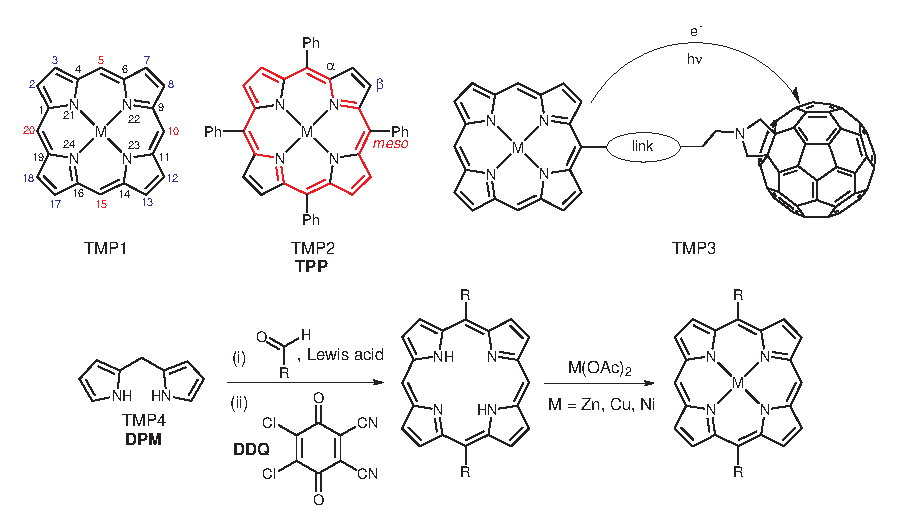
\includegraphics{figures/intro/porphyrin-numbering.eps} 
		\caption[]{(top) Examples of porphyrins: \cmpd{porphine} is porphine, with IUPAC atom numbering indicated; \cmpd{tpp} is tetraphenylporphyrin (TPP), with the [18]-annulene aromatic circuit indicated in red, and with the `common names' for the atomic positions; \cmpd{dyad} is a schematic example of a \ce{C60}--porphyrin dyad, in which absorption of a photon of light can result in charge separation. (bottom) Example of porphyrin synthesis by condensation of an aldehyde with DPM \cmpd{dpm}, followed by oxidation with DDQ\@. Metal insertion then follows.}
		\label{fig:intro:porphs}
	\end{figure}


	The introduction of a central metal ion into a porphyrin, which acts as a square planar tetradentate ligand, allows further modulation of the porphyrin's properties. For example, a nickel(II) porphyrin \cmpd{switch} has been used as a photochemical spin switch, where the action of the azobenzene photoswitch causes an axial pyridine to coordinate to the Ni(II), changing it from low spin ($S=0$) to high spin ($S=1$) (\autoref{fig:intro:switches}).\autocite{Venkataramani2011} Copper(II) porphyrins are paramagnetic; they have been explored for their applications as biochemical distance rulers by double electron-electron resonance (DEER\nomenclature{DEER}{Double electron-electron resonance}).\autocite{Bowen2016} Axial coordination of ligands to metalloporphyrins, yielding square pyramidal or octahedral coordination geometries, is useful for the synthesis of supramolecular assemblies (\autoref{fig:intro:porphy-supra}), as has been recently reviewed.\autocite{Wang2016}

	\begin{figure}[ht!]
		\replacecmpd{switch}
		\centering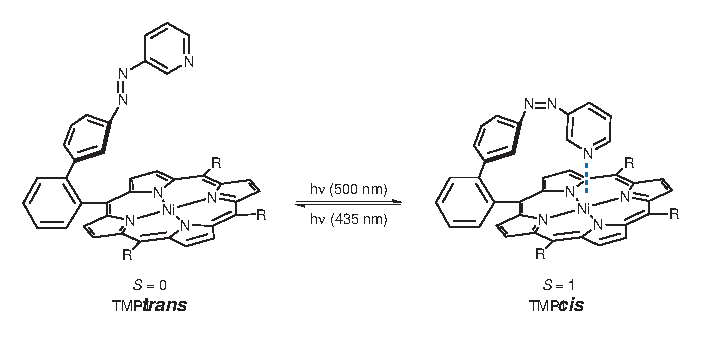
\includegraphics{figures/intro/switch.eps} 
		\caption[]{A photochemically mediated spin switch employing an azobenzene link which, upon irradiation with \SI{500}{\nano\metre} light, undergoes a \textit{trans}--\textit{cis} isomerism, causing a pyridine ligand to axially coordinate the Ni(II) and switching the spin state from low spin (\textit{\textbf{trans}}) to high spin (\textit{\textbf{cis}}).\autocite{Venkataramani2011}}
		\label{fig:intro:switches}
	\end{figure}

	This thesis concerns the chemistry of butadiyne-linked zinc-porphyrin oligomers. This class of oligomer was first prepared by Arnold in 1978,\autocite{Arnold1978} and has since been the subject of intense study, mainly by his group and that of Anderson.\autocite{Arnold1992,Arnold2000,Anderson1994,Anderson1999} Historically, Arnold focused primarily on the physical properties of short oligomers (\ltt{e.g.} porphyrin dimers),\autocite{Arnold2000} whilst Anderson explored the supramolecular chemistry of porphyrins. The Anderson group has prepared spectacular structures such as porphyrin ladders,\autocite{Taylor1999} the nanoring-template complex \rwt6,\autocite{Hoffmann2008} the Vernier-templated figure-of-eight \cp{12}$\bullet{}$\temp{6\tsub2},\autocite{OSullivan2011} ring-in-ring complexes,\autocite{Rousseaux2015} and an axially elongated nanoring tube \tubewt{} (\autoref{fig:intro:porphy-supra}).\autocite{Neuhaus2015} The preparation of these structures has relied on the binding of nitrogenous ligands -- typically pyridine -- to the axial coordination site of the Zn-porphyrin. The Zn-porphyrin--pyridine binding constant is weak ($K = 10^4\ \si{\per\Molar}$),\autocite{Cole1972} but chelate cooperativity diminishes the entropic cost for multiple-binding, leading to huge binding constants.\autocite{Hogben2011} For example, \temp6 in \rwt6 has a binding constant of $K = 10^{36}\ \si{\per\Molar}$.\autocite{Hoffmann2008} The butadiyne link ensures good conjugation between the porphyrin units, which can readily adopt a coplanar conformation without steric hindrance, in contrast to the steric clash between porphyrin $\beta$-protons in a planar monoalkyne-linked dimer. However, as we will see in \autoref{ch:dimer}, there is little thermodynamic preference for planarity: the barrier to torsional rotation in a butadiyne-linked porphyrin dimer is about \SI{2}{\kilo\joule\per\mole}.\autocite{Winters2007,Peeks2016} As such, butadiyne-linked porphyrin oligomers are prone to the introduction of conjugation-breaking defects in the form of non-planarity of adjacent porphyrin units. 


	\begin{figure}[ht!]
		\centering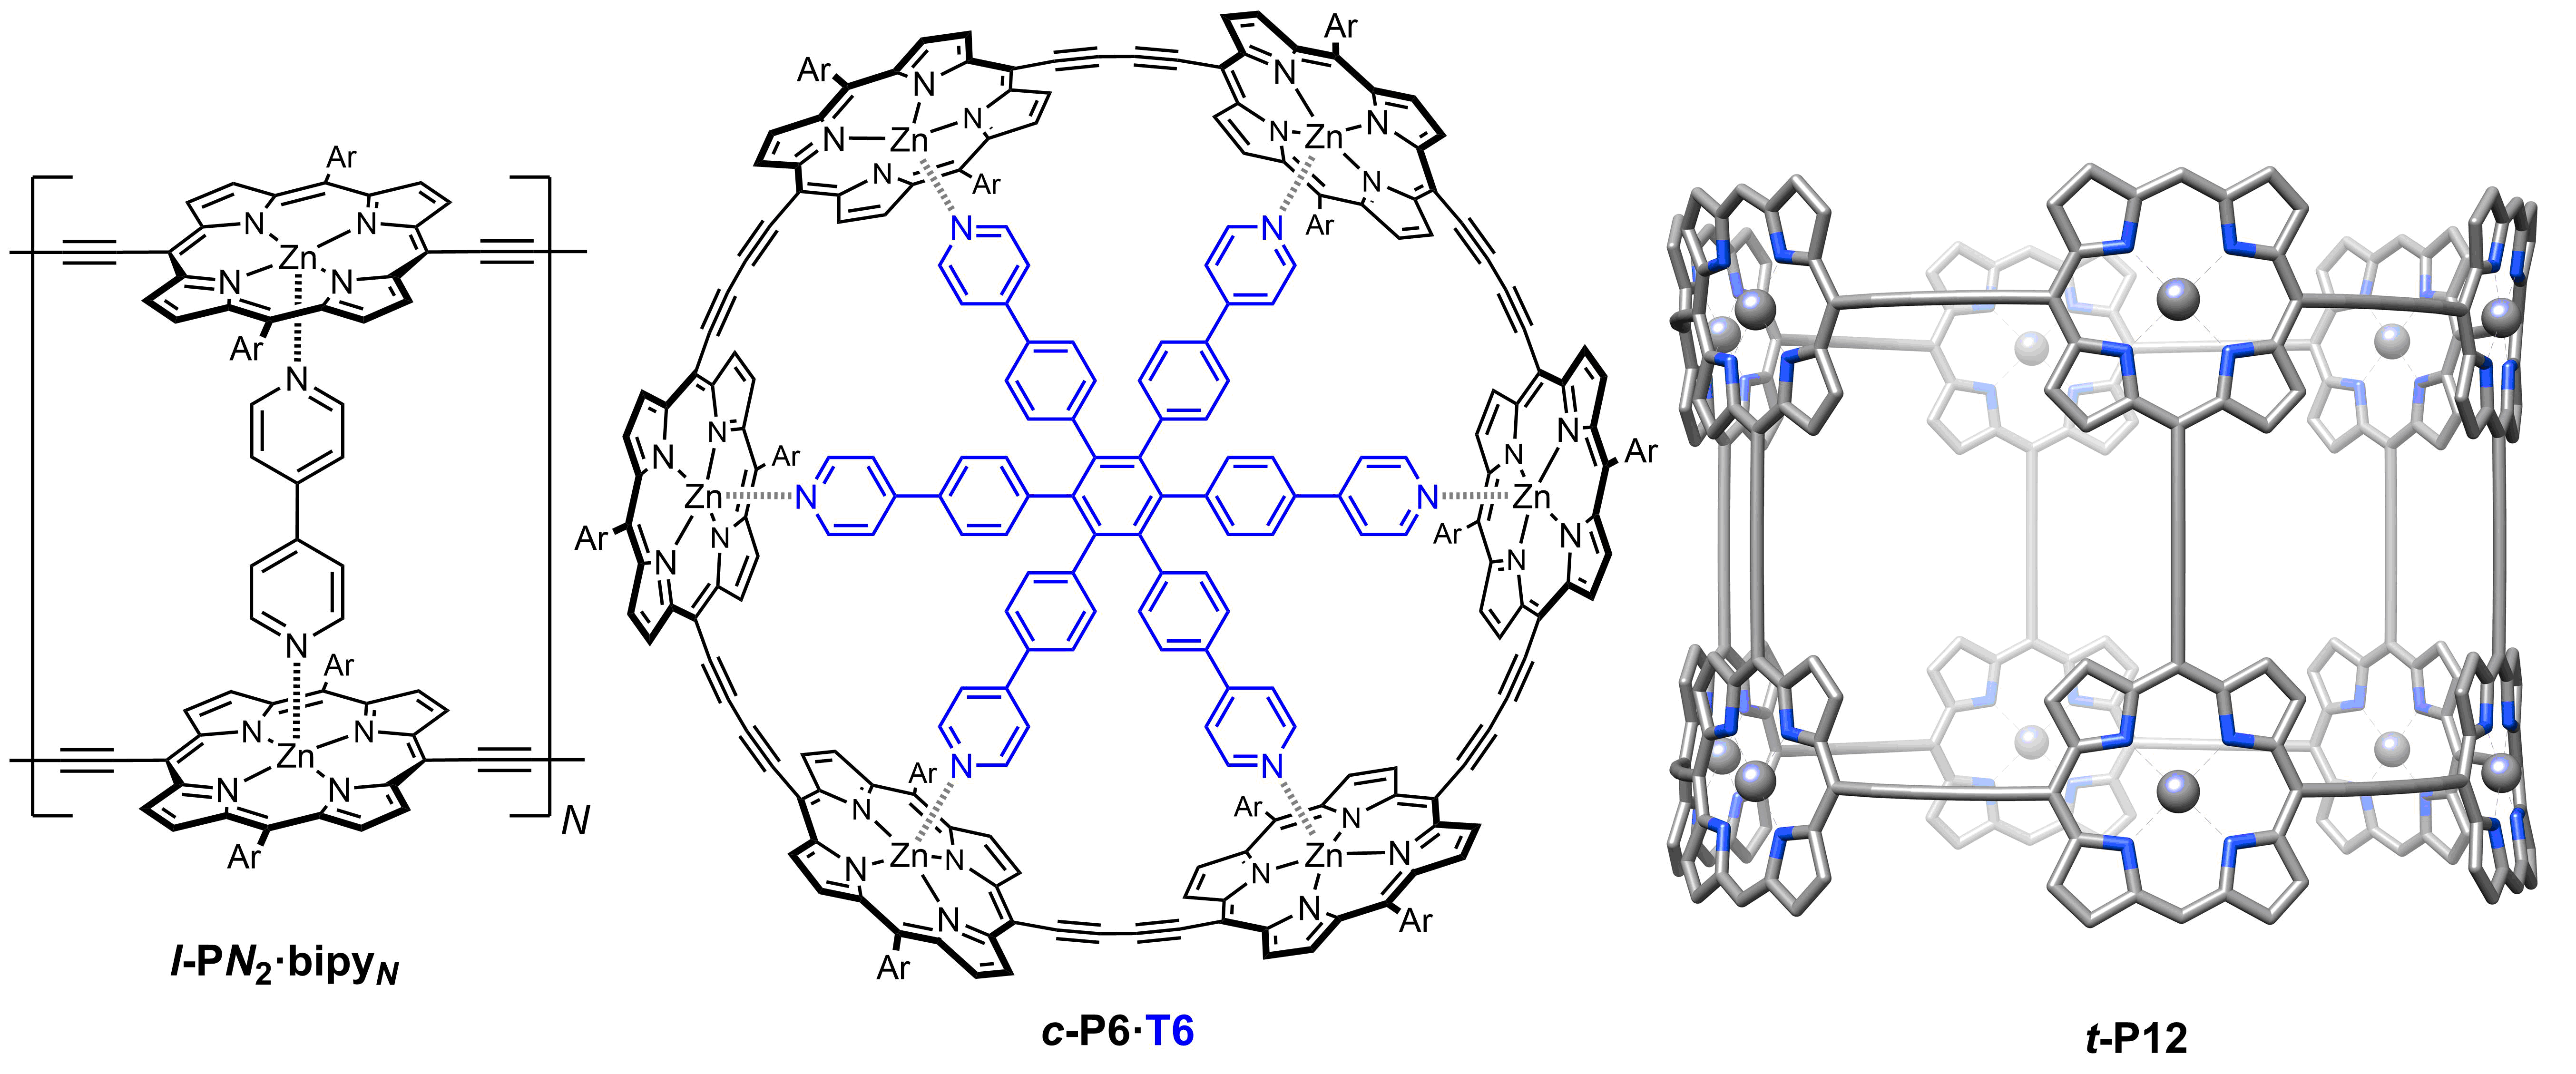
\includegraphics[width=\textwidth]{figures/intro/porphy-supra.png} 
		\caption[]{A double-stranded porphyrin ladder formed by coordination of 4,4\tsup{\textprime{}}-bipyridine (bipy\nomenclature{bipy}{4,4\tsup{\textprime{}}-Bipyridine}),\autocite{Taylor1999} a [6]-porphyrin nanoring \rwt6,\autocite{Hoffmann2008} and a [12]-porphyrin nanotube (BLYP/6-31G*) \tp{12}.\autocite{Neuhaus2015}}
		\label{fig:intro:porphy-supra}
	\end{figure}


	\begin{figure}[ht!]
		\centering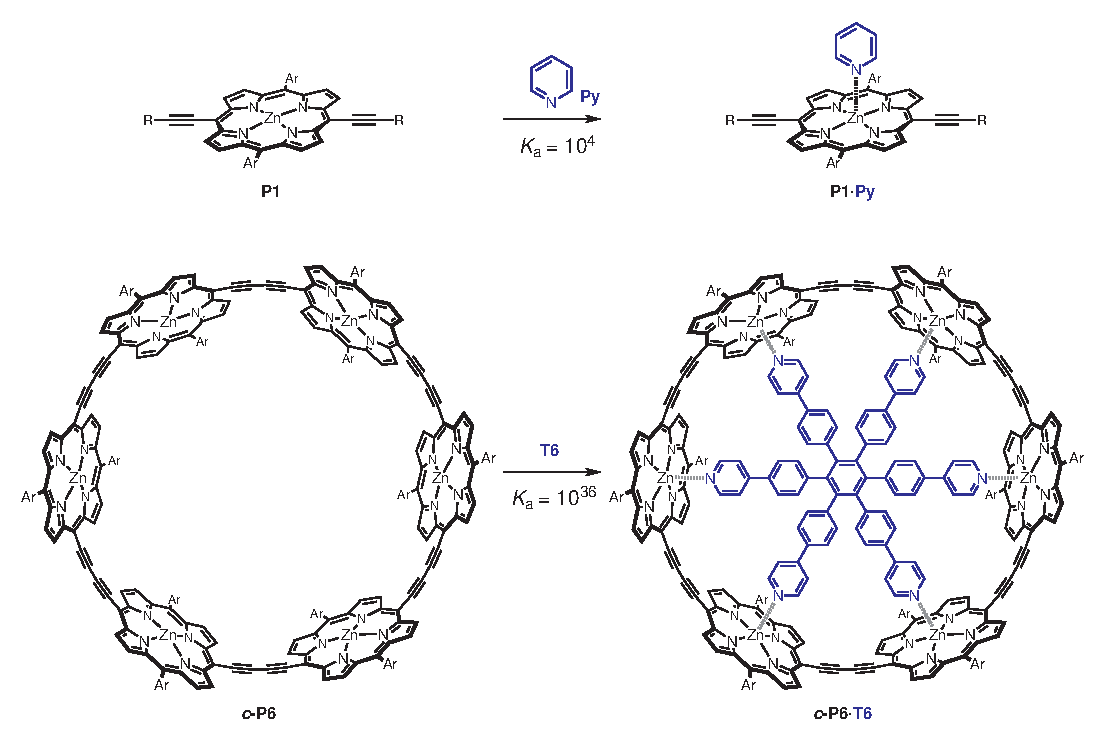
\includegraphics[width=\textwidth]{figures/intro/porphy-binding.eps} 
		\caption[]{Comparison of binding constants for a porphyrin monomer to pyridine and for a [6]-porphyrin nanoring \cp6 to a hexadentate template \temp6, demonstrating significant cooperativity in the latter.}
		\label{fig:intro:porphy-binding}
	\end{figure}



	The high absorption coefficients of porphyrins and their oligomers often motivate comparisons to the light harvesting complexes in green plants, which comprise circular arrays of chlorophyll molecules.\autocite{VanGrondelle1994,McDermott1995} Efforts continue to use porphyrins in high-efficiency dye-sensitised solar cells (DSSCs)\nomenclature{DSSC}{Dye-sensitised solar cell}, through both the design of new materials and investigations into electron transport properties.\autocite{Higashino2015,Gilbert2015} To date, the power conversion efficiency of synthetic DSSCs has reached 12\%, compared to 22\% for leading perovskite materials and 26\% for silicon cells.\autocite{NREL2016} The theoretical limit for a single-junction cell, the Shockley-Queisser limit, is 34\%.\autocite{Shockley1961} Porphyrins have found more application in medicine, where they are employed for photodynamic therapy (PDT\nomenclature{PDT}{Photodynamic therapy}). In this treatment for cancer, a sensitiser molecule (porphyrin) accumulates in a tumour and is then irradiated with light. Intersystem crossing to the triplet manifold occurs, resulting in sensitisation of oxygen and oxidative destruction of tissue.\autocite{Mody2000,Ethirajan2011}

	The field of porphyrin chemistry is broadened by the introduction of the porphyrinoids and the expanded and contracted porphyrins.\autocite{Stepien2011,Mack2016} These molecules are essentially variations upon the theme of the porphyrin: for example, diverse porphyrinoids can be generated by replacing the pyrroles of the macrocycle with other 5-membered aromatic rings, like furan or thiophene.\autocite{Vogel1989,Vogel2000} Expanded porphyrins (\ltt{e.g.} \cmpd{osuka52}, \autoref{fig:intro:osuka}) are simply large porphyrinoids, with at least 17 atoms in their `internal ring pathway'.\autocite{Sessler2003,Saito2011} The diversity of porphyrinoids has proven extremely useful for dissecting concepts in aromaticity,\autocite{Osuka2011,Stepien2011,Wu2013,Pawlicki2015} including excited state and M\"obius aromaticity, as we shall see in the next section. 

	\begin{figure}[ht!]
		\replacecmpd{osuka52}
		\centering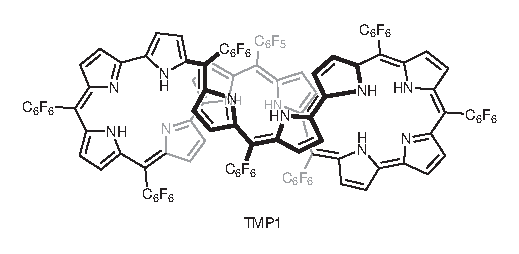
\includegraphics{figures/intro/osuka.eps} 
		\caption[]{Osuka's H\"uckel aromatic [50]-\pii{} expanded porphyrin \cmpd{osuka52}.\autocite{Soya2015}}
		\label{fig:intro:osuka}
	\end{figure}

\FloatBarrier

\section{Aromaticity}
	Aromaticity is a heavily-reviewed topic, and was the subject of entire issues of \textit{Chem. Rev.} in 2001 and 2005,\autocite{Schleyer2001,Schleyer2005} and of \textit{Chem. Soc. Rev.} in 2015.\autocite{Martin2015} In this section, a brief historical account of aromaticity will be given, illustrated by prominent examples. 

	A simple bibliometric analysis using Google Books\autocite{Michel2011} shows that, although benzene was widely written about from the late 1800s, the concept of `aromaticity' only gained prominence with the appearance of molecular orbital theory, ring current theories, and NMR (\autoref{fig:intro:ngram}a, nuclear magnetic resonance). This correlation describes the development of aromatic chemistry, from the study of compounds with particular olfactory properties to the broad-ranging subject of aromaticity, facilitated by synthetic, spectroscopic, and computational advances. 

		\begin{figure}[ht!]
			\centering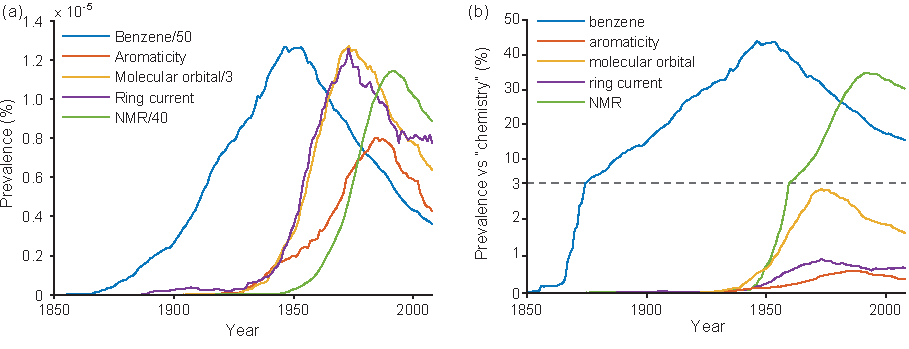
\includegraphics{figures/intro/ngram.pdf} 
			\caption[]{Bibliometric analysis (ngrams)\autocite{Michel2011} showing the use of benzene, aromaticity, molecular orbital, ring current and NMR in the English language corpus of Google Books.\autocite{Michel2011} In (a) the prevalence of each phrase, case insensitive, is shown. The numbers in the legends denote a scale factor applied to the specified term. In (b) the prevalence of the (case sensitive) terms relative to the prevalence of the word `chemistry' are shown. All data are smoothed with a 10-point (21-year) moving average.}
			\label{fig:intro:ngram}
		\end{figure}

	The decline in frequency in all of these terms since the mid-1900s is partly a consequence of chemistry forming a smaller part of the English language corpus in modern times. In \autoref{fig:intro:ngram}b, the frequencies of several terms relating to aromaticity are normalised by the frequency of the word `chemistry'. The results show that relative to chemistry, interest in ring currents and aromaticity has remained fairly steady since the 1980s. It is reflective of benzene's importance that in the 1940s, the word `benzene' was mentioned almost half as many times as the word `chemistry'!

	\subsection{Early aromaticity}

		Benzene (\cmpd{benzene}, \autoref{fig:intro:aromatics}) was isolated by Faraday in 1825, but its structure remained unknown until the 1860s. After Kekul\'e and Coupers' independent realisations that carbon is tetravalent,\autocite{Kekule1858,couper1858nouvelle} the former deduced (through the famous, perhaps apocryphal, day-dream of a snake biting its own tail) that benzene is cyclic.\autocite{kekule1865constitution} Kekul\'e proposed a benzene structure with alternating single and double bonds, which he later refined by the suggestion that the single and double bonds rapidly interconverted.\autocite{kekule1866untersuchungen} Benzene and the other aromatic molecules became defined by reactivity, most notably by the fact that they underwent a substitution reaction with bromine, as opposed to the addition expected for alkenes (\autoref{fig:intro:arom-rx}). 

		\begin{figure}[ht!]
			\replacecmpd{benzene}
			\replacecmpd{cot}
			\replacecmpd{cbd} 
			\replacecmpd{tenannulene}
			\replacecmpd{homoarom}
			\replacecmpd{trishomoarom}
			\centering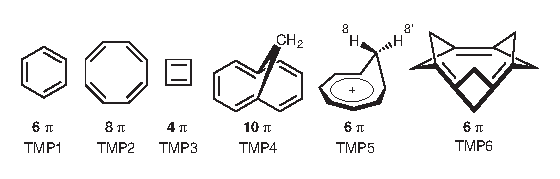
\includegraphics{figures/intro/aromatics.eps} 
			\caption[]{Examples of aromatic, non-aromatic, and antiaromatic compounds.}
			\label{fig:intro:aromatics}
		\end{figure}

		\begin{figure}[ht!]
			\centering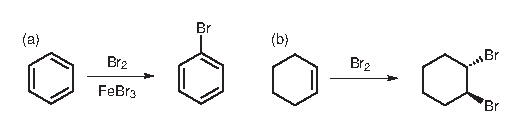
\includegraphics{figures/intro/arom-rx.eps} 
			\caption[]{(a) Benzene undergoes a substitution reaction with bromine, in the presence of \ce{FeBr3} as an activating Lewis Acid; (b) cyclohexene undergoes an addition reaction with benzene.}
			\label{fig:intro:arom-rx}
		\end{figure}

		Thiele proposed a theory to account for this reactivity, namely that unsaturated carbons had a `partial valence', which was especially reactive.\autocite{Thiele1899} Adjacent pairs of partial valences could interact with (saturate) each other, provided neither was at a terminal position (hence, the partial valences in ethylene could not saturate). Reactivity was thus found at the unsaturated partial valences, explaining the reactivity at the 1,4-positions of 1,3-butadiene and the stability of benzene (\autoref{fig:intro:thiele}). However, Thiele's theory was proven wrong by our earlier hero of chlorophyll chemistry, Willst\"atter, who isolated cyclooctatetraene (COT\nomenclature{COT}{Cyclooctatetraene}, \cmpd{cot}) in 1911,\autocite{Willstatter1911} and found that it reacted with bromine as an alkene, without any hint of partial valence stabilisation.

		\begin{figure}[ht!]
			\centering
\includegraphics{figures/intro/thiele-valence.eps} 
			\caption[]{Thiele's theory of partial valences applied to (a) ethylene, (b) 1,3-butadiene and (c) benzene. Partial valences are indicated by dotted lines: blue dotted lines are unsatisfied partial valences, and thus sites of high reactivity. Saturated partial valences are denoted by red dotted semicircles: these positions are unreactive.}
			\label{fig:intro:thiele}
		\end{figure}

		Although much research into aromatic compounds continued in the latter part of the 19\nth century, heavily motivated by their application in dyestuffs, the notion of aromaticity as a distinct chemical property did not really exist until the 1930s, with the development of molecular orbital theory, and only became ascendant as late as the 1950s (\autoref{fig:intro:ngram}). %Amusingly, a statement by Gilman and Towne on (super-)aromaticity in 1932 would not be out of place in a review published today:\autocite{Gilman1932}

		%\begin{quote}
		%	Aromatic properties are the peculiar properties exhibited by aromatic compounds. Actually, there is no agreement as to what constitutes aromatic compounds or aromatic properties. We do not know exactly what peculiarities in unsaturation are necessary to give a cyclic compound aromatic properties. Nor is there concordance of opinion as to the particular properties which are characteristic of aromatic compounds.
		%\end{quote}

	\subsection{The aromatic sextet and H\"uckel's theory}

		Crocker, Armit and Robinson presented the idea of the \textit{aromatic sextet} in the 1920s, proposing that benzene's aromatic stability arose from the favourability of a sextet of valence electrons.\autocite{Crocker1922,Armit1925,Balaban2005} Pauling and Wheland soon developed valence bond (VB) theory and the accompanying notion of resonance was quickly adopted by organic chemists. Benzene's aromatic stabilisation was explained by the presence of multiple resonance structures, in which the delocalised \pii{}-electrons are represented by different VB representations: more resonance structures confer more stability.\autocite{pauling1933nature} Although Erich H\"uckel's molecular orbital (MO) theory was developed in the 1930s, and was able to quantitatively explain the stability of aromatic molecules, his explanations struggled to displace the pervasive and simple resonance theory.\autocite{huckel1937grundzuge,berson1999chemical} It was really only with the development of mnemonics, such as Doering's presentation of the $[4n+2]$ rule\autocite{Doering1951} (bringing the theory back to aromatic sextets) and Frost and Musulin's graphical presentation of H\"uckel's orbital energies\autocite{Frost1953} that H\"uckel's MO theory entered the mainstream.\autocite{berson1999chemical} The familiar $[4n+2]$ rule states that a molecule with $[4n+2]$ conjugated \pii{}-electrons is aromatic, while a molecule with $[4n]$ \pii{}-electrons is antiaromatic, where $n$ is a non-negative integer. 

		By constructing the Frost-Musulin diagrams for benzene and cyclobutadiene (CBD\nomenclature{CBD}{Cyclobutadiene}, antiaromatic, \cmpd{cbd})  we can immediately see that benzene, in a \symm{D}{6h} model, has a filled degenerate pair of orbitals as its highest-occupied MO (HOMO), whereas CBD, with only $[4n]$ \pii{}-electrons, adopts a triplet configuration in its \symm{D}{4h} symmetric structure (\autoref{fig:intro:huckel}). Further calculations reveal that CBD is better described as a \symm{D}{2h} rectangle, with increased double-bond and single-bond character (\ltt{i.e.} bond length alternation, BLA) compared to benzene.\autocite{Bally1980} This pseudo-Jahn-Teller (PJT\nomenclature{PJT}{Pseudo-Jahn-Teller})\autocite{Kertesz2005} distortion is common to the $[4n]$-\pii{} antiaromatic molecules, and lifts the HOMO degeneracy as shown in \autoref{fig:intro:huckel}, leading to a closed shell antiaromatic configuration with a small HOMO--LUMO (lowest unoccupied MO) gap.

		\begin{figure}[ht!]
			\centering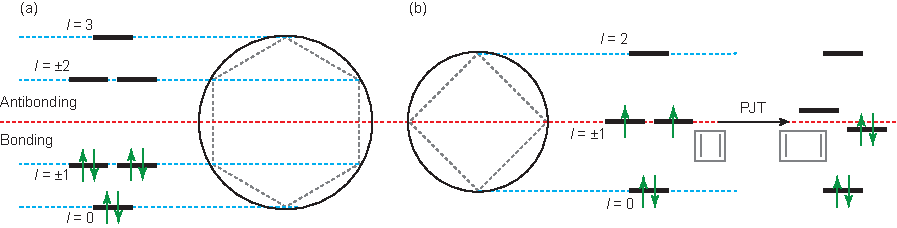
\includegraphics{figures/intro/huckel.pdf} 
			\caption[]{Frost-Musulin diagrams for (a) benzene and (b) CBD\@. In (a), all of the bonding orbitals (below the horizontal red line) of benzene are filled. In (b), the half-occupied degenerate pair is non-bonding. A pseudo-Jahn-Teller (PJT) distortion breaks the degeneracy and leads to a bonding character for one electron pair.}
			\label{fig:intro:huckel}
		\end{figure}

		\FloatBarrier

	\subsection{Ring currents}

		In addition to advances in theory, the early part of the 20\nth century saw a development of experimental methods for the quantification of aromaticity. Pascal noted that aromatic molecules were more diamagnetic ($\chi_\text{M}$) than expected on the basis of additive substituent contributions ($\chi_{\text{M}}^\prime{}$),\autocite{pascal1910magnetochemical} and Pacault termed this excess of diamagnetic susceptibility the `exaltation' ($\Lambda$).\autocite{Pacault1961,Gleiter2012} 

		\begin{equation}
			\Lambda = \chi_\text{M} - \chi_{\text{M}}^\prime{}
		\end{equation}

		The utility of exaltation measurements for the assignment of aromaticity was demonstrated by Dauben \ltt{et al.} in 1969,\autocite{Dauben1969} but by this time there was a more experimentally informative, and appealing, method of measuring magnetic properties: NMR\@. Nowadays, susceptibility measurements have almost entirely fallen out of favour,\autocite{Gershoni-Poranne2015} despite the fact that they were once described as the `only' unambiguous assignor of aromaticity.\autocite{Schleyer1996a}

		NMR is a particularly helpful descriptor of aromaticity because of the effect of so-called aromatic ring-currents on NMR chemical shifts. The resonances of nuclei inside an aromatic ring are shielded; those outside are deshielded. For example, the protons of benzene are deshielded from an olefinic chemical shift (5~ppm)\nomenclature{ppm}{Parts per million} to what is now colloquially called `the aromatic region', around 7~ppm. In the ring-current model (RCM)\nomenclature{RCM}{Ring-current model} the delocalised \pii{}-electrons in an aromatic ring precess about the ring centre in the presence of an external magnetic field $B_\text{ext}$ (typically defined along the $z$ axis, perpendicular to the molecular plane). This precession is a \textit{diatropic} current of electrons which flows clockwise around the ring, when viewed from the $z$ axis (looking towards $-z$) (\autoref{fig:intro:ringcurr}). Consistent with Amp\`ere's right hand screw rule, this induced ring-current $J_\text{ind}$ has an associated magnetic field $B_\text{ind}$, which opposes $B_\text{ext}$ inside the ring (hence has a shielding effect) and reinforces $B_\text{ext}$ outside the ring (hence deshielding). Examples of the shielding and deshielding effects arising from the RCM will be discussed shortly, but first we must give a surprisingly late introduction to antiaromaticity, via the annulenes.

		\begin{figure}[ht!]
			\centering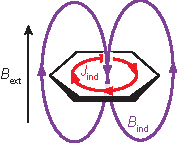
\includegraphics{figures/intro/ring-current.pdf} 
			\caption[]{Representation of the induced ring current ($J_\text{ind}$) in benzene in the presence of an applied magnetic field  ($B_\text{ext}$). The induced current generates its own magnetic field, $B_\text{ind}$ which opposes $B_\text{ext}$ inside the ring, and reinforces it outside.}
			\label{fig:intro:ringcurr}
		\end{figure}

		Benzene, COT and CBD are all members of the class of molecules termed the \textit{annulenes} by Sondheimer.\autocite{Sondheimer1962} Annulenes are ring systems of general formula C\tsub{\textit{m}}H\tsub{\textit{m}} comprising alternating single and double C--C bonds. Sondheimer prepared a spectacular array of annulenes and dehydroannulenes, in which some \ce{C=C} bonds are replaced with \ce{C#C} bonds.\autocite{Sondheimer1963,Sondheimer1967,Sondheimer1972} He made the remarkable discovery that while the $[4n+2]$-annulenes exhibited NMR spectra similar to that of benzene: \ltt{i.e.} shielded inner resonances and deshielded outer resonances, the $[4n]$-annulenes had reversed spectra: inner resonances were deshielded and outer resonances shielded.\autocite{Sondheimer1967} 

		The term \textit{antiaromatic} was first applied by Breslow in 1965 to describe the instability exhibited by some molecules with $[4n]$ \pii{}-electrons, antithetical to the established aromatic stabilisation of $[4n+2]$-\pii{} molecules.\autocite{Breslow1965} In antiaromatic molecules, the ring current flows in the opposite direction (\textit{paratropic}) to that in aromatic molecules,\autocite{Steiner2001} which accounts for the opposite effects on chemical shifts.

		It is important to note that both aromatic and antiaromatic molecules simultaneously possess counter-rotating diatropic and paratropic ring current character to different extents. The diatropic ring current (and the diamagnetic susceptibility) is a ground state property; paratropic currents (and temperature-independent paramagnetic susceptibility) arise from interactions with excited states.\autocite{Longuet-Higgins1967} It is easy to see why the paratropic currents can dominate for antiaromatic molecules due to the smaller HOMO-LUMO gap. 

		In a H\"uckel theory approximation, a symmetric annulene has a manifold of \pii{}-orbitals with angular momentum values $l = 0, \pm{}1, \pm{}2 \mathellipsis{}$. For aromatic molecules with $[4n+2]$ \pii{}-electrons, these orbitals are filled to $l=\pm n$. In the antiaromatic case, the degenerate pair $l=\pm n$ is only half-filled, and can undergo distortions to lift the $l=\pm n$ degeneracy and afford a HOMO with $l = n$ and LUMO with $l = -n$. The HOMO--LUMO gap is small in this case, compared to that for an aromatic molecule (\autoref{fig:intro:huckel}), so the excited state transition (and accompanying change in angular momentum) which induces the paratropic ring currents is more accessible.\autocite{Longuet-Higgins1967,Pople1966} 

		Fowler and Steiner have presented an alternative model in which the ring current direction is predicted by the symmetry of the dominant frontier-orbital transitions -- in this model, both diatropic and paratropic ring currents arise from transitions to excited states. A rotationally allowed transition (as between a Jahn-Teller distorted angular-momentum pair) leads to a paratropic current, while a translationally allowed transition (as between $l=\pm{}n$ and $l=\pm [n+1]$) leads to diatropicity.\autocite{Fowler2001,Steiner2001} More thorough introductions to the quantum mechanical origin of ring currents and magnetic susceptibilities can be found in the cited reviews and references therein.\autocite{Lazzeretti2000,Gomes2001}

	 	The NMR shielding effect inside an aromatic ring can be probed by molecules where an NMR-active nucleus is located inside the ring. Vogel and coworkers were able to synthesise a [10]-annulene derivative with a methylene bridge above the annulene plane (1,6-methanocyclodecapentaene, \cmpd{tenannulene}): as expected from the RCM, this methylene is shielded by about \SIrange{2}{3}{\ppm} to \SI{-0.5}{\ppm}.\autocite{Vogel1967} The propensity of \ce{Li+} to coordinate to the \pii{}-systems of aromatic molecules can also be exploited, allowing the use of \nmriso{7}{Li} NMR to measure the ring-current shielding effect.\autocite{Schleyer1996a}

	 	Porphyrin chemistry provides many examples of the ring current shielding effects for aromatic and antiaromatic derivatives. The porphine ligand is formally in a $2-$ oxidation state with an aromatic set of $18$ \pii{}-electrons. Typically, a $2+$ metal binds to the porphyrin to give a net zero charge, as is the case for M = Zn, Mg, Ni, 2H, \ltt{etc}. In the latter case, M = 2H, the protons are characteristically shielded from a pyrrolic \SI{8}{\ppm} to \SI{-2}{\ppm}. Vaid and coworkers have prepared a TPP complex of Si, where the TPP ligand has a $-4$ ($20\pi$) oxidation state. \nmriso{29}{Si} NMR shows that the central Si is deshielded by \SI{125}{\ppm} on account of the antiaromatic ring-current.\autocite{Cissell2005}

	\subsection{Other experimental signs of aromaticity}
		
		There are other properties available by which to assign aromaticity. The most traditional of these is based on aromatic reactivity: a propensity to undergo electrophilic aromatic substitution rather than addition. A related aspect is the energetic stability of aromatic systems, arising from a large resonance stabilisation energy (contrast to zero, or negative, stabilisation for antiaromatic systems). Finally, structural properties can support an assignment of aromaticity: aromatic compounds exhibit a low BLA, whereas the pseudo-Jahn-Teller distortion for antiaromatic compounds leads to a higher BLA\@. Such data can come from infra-red (IR) or Raman spectroscopies, X-ray diffraction, or from calculation.% In the case of benzene, its planar hexagonal structure was confirmed by crystallography of hexamethylbenzene reported by Lonsdale in 1929.\autocite{Lonsdale1929}

	\subsection{Predicting aromaticity}

		There is a multitude of methods available to computationally predict and characterise aromaticity in molecules. Their utility is facilitated by the availability of computing power and the applicability of density functional theory (DFT), which scales well for small molecules (systems with a few hundred atoms are routine) with generally accurate results.



		\subsubsection{Ring currents}\label{sec:intro:rc}

			Perhaps the most popular methods for predicting aromaticity are those which measure the properties of the aromatic ring current. The first of these techniques was the nucleus independent chemical shift (NICS), which evaluates the NMR shielding at a point in space around a molecule. This is achieved by placing a `ghost' atom (in Gaussian, `Bq', after the character (latterly a ghost) Banquo\autocite{shakespeare1903macbeth} in \textit{Macbeth}) at the desired probe position(s). In the first reported NICS calculations, the ghost atoms were placed at the geometric centres of rings.\autocite{Schleyer1996} For some inorganic ring systems, it was noted that the in-plane NICS was prone to contamination by $\sigma$ and in-plane \pii bonds, motivating the dissection of \pii and $\sigma$ components to give NICS\tsub{\pii} and NICS\tsub{$\sigma$}.\autocite{Schleyer1997} The measurement of NICS($X$) at some position $X$ \si{\angstrom} above the ring plane was also used for these inorganic systems, to avoid in-plane contributions.\autocite{Schleyer1997} Indeed, it had been earlier noted that NICS values were higher above the ring plane than in the plane for small \pii{}-aromatic systems, reflecting the toroidal distribution of \pii{}-electrons and the presence of $\sigma$ bond anisotropy contamination for in-plane measurements.\autocite{Schleyer1996} 

			In addition to choosing a suitable $z$-axis height, the selection of the correct tensor component to describe aromaticity is also important: the original report used the isotropic (iso) shielding (NICS\tsub{iso}),\autocite{Schleyer1996} but later studies have placed increased emphasis on the $zz$ shielding tensor component (NICS\tsub{$zz$}) as being more reflective of aromaticity effects. Of the myriad combinations of `dissected NICS' (\ltt{i.e.} \pii contributions only), distances above the ring plane, and tensor components, it was found that NICS(0)\tsub{$\pi zz$} gave the best correlation to aromatic stabilisation energy, and that the non-dissected NICS(1)\tsub{$zz$} was a suitable alternative, since shifting the ghost atom \SI{1}{\angstrom} above the ring plane has the effect of removing most in-plane contamination.

			Since its invention in the late 1990s the NICS method has been extended to the calculation of shielding isosurfaces\autocite{Klod2001} and NICS-scans\autocite{Gershoni-Poranne2014} which reveal the variation in aromaticity in different parts of a molecule.\autocite{Stanger2006,Gershoni-Poranne2014} Examples of the utility of NICS and its derivatives have been thoroughly reviewed.\autocite{Chen2005,Gershoni-Poranne2015} 

			NICS evaluates the effects of the ring current: the magnetic shielding and deshielding. It is also possible to computationally predict and visualise the ring current. The anisotropy of the induced current density (ACID) method depicts the induced current as an isosurface around the molecule.\autocite{Herges2001} By examining this anisotropy property, rather than just the current density field, it is possible to subtract out local diamagnetic (isotropic) atomic ring currents, which otherwise dominate. As a result, electron delocalisation can be visualised as a three-dimensional isosurface around the molecule (\autoref{fig:intro:acid}).

			\begin{figure}[ht!]
				\centering\includegraphics{figures/intro/acid.pdf} 
				\caption[]{ACID isosurfaces (yellow, isovalue = 0.05) and current vectors (green/red) for (a) benzene and (b) a zinc porphyrin monomer. The monomer is substituted with trimethylsilylacetylenes. B3LYP/6-31G* (LANL2DZ ECP for Zn). The current vectors are calculated for an applied magnetic field perpendicular to the aromatic ring planes (\ltt{i.e.} out of the page).}
				\label{fig:intro:acid}
			\end{figure}


			ACID was first applied by Wallenborn \ltt{et al.} to assess transition state aromaticity,\autocite{Wallenborn1998} and the utility of the technique was significantly broadened from aromaticity to other examples of conjugation, including hyperconjugation and spiroconjugation, by Herges \ltt{et al}.\autocite{Herges2001,Geuenich2005} An illustrative example of ACID's application to porphyrin ring currents shows the utility of the technique in dissecting electron delocalisation pathways.\autocite{Wu2013} The additional calculation of induced current vectors shows the direction of electron flow in the presence of an applied field, and thus the assignment of diatropic and paratropic ring currents.\autocite{Geuenich2005}

			It is also possible to directly calculate the magnitude of the ring current passing through a given bond. The Gauge-Including Magnetically Induced Currents (GIMIC) technique is popular for this calculation, and several examples of its use have been reported.\autocite{GIMIC2004,Fliegl2009,Fliegl2012}


		
		\subsubsection{Structural}

			In benzene, all of the \ce{C-C} bonds are of equal length: there is no BLA, indicating complete electron delocalisation. The extent of BLA in a molecule can be quantified using the harmonic oscillator model of aromaticity (HOMA\nomenclature{HOMA}{Harmonic oscillator model of aromaticity})\autocite{Kruszewski1972}

			\begin{align}
				\text{HOMA} &= 1 - \left[\frac{\alpha}{N} \sum_i^N ( R_\text{opt} - R_\text{i})^2\right] \\
				&= 1 - \alpha (R_\text{opt} - R_\text{av})^2 - \frac{\alpha}{N} \sum_i^N( R_\text{av} - R_\text{i})^2 \\
				&= 1 - \text{EN} - \text{GEO}
			\end{align}

			\noindent{}where HOMA is a quantity from 0 (complete localisation) to 1 (complete delocalisation), $\alpha$ is an empirical scaling constant, $N$ is the number of bonds over which the sums run, $R_\text{i}$ is the length of the i\nth bond, $R_\text{av}$ is the average bond length, and $R_\text{opt}$ is the optimum bond length for a fully delocalised bond (\ltt{e.g.} \SI{1.388}{\angstrom} for \ce{C-C}).\autocite{Kruszewski1972} In other words, the first term (EN) relates to an increase (\ltt{vs.} the optimum) in mean bond length in the system, and the second term (GEO) relates to the amount of BLA\@. Both of these parameters indicate non-aromaticity, and hence a decrease in HOMA towards zero.\autocite{Krygowski2000a}

			The theory and application of structural descriptors of aromaticity have been reviewed by Krysowski and Cyra\'nski.\autocite{Krygowski2001} Although BLA is a good metric for aromaticity in small molecules, it has been shown computationally that [30]-annulene exhibits the magnetic characteristics of aromaticity despite the presence of significant BLA, and even larger annulenes (up to [66]-annulene) are aromatic if high symmetry (\symm{D}{6h}) is retained.\autocite{Wannere2003,Choi1998}

		\subsubsection{Energetic}

			The increased thermodynamic stability conferred by aromaticity is often termed the aromatic stabilisation energy (ASE), and can be calculated explicitly. The forerunners of the ASE methods were estimations of resonance energy, either by experiment or calculation.\autocite{Gleiter2012,Cyranski2005}

			In calculations of resonance energy, the additional stabilisation of aromaticity is taken as the difference between the aromatic molecule's energy and the energies of the substituent `localised' components. For example, the resonance energy of benzene can be estimated by the difference of benzene's electron energy and the sum of its bond contributions: three \ce{C=C}, three \ce{C-C} and six \ce{C-H}. These approaches require the energy of the aromatic molecule, and reliable energies for the localised substituents.

			The calculation of ASE depends on devising, and calculating, a suitable reaction scheme which directly reports on the aromaticity of the molecule, whilst avoiding contributions to the reaction energy from changes in hybridisation or atom numbers. The two primary methods are the homodesmotic stabilisation energy (HSE) and its improved form: the isomerisation stabilisation energy (ISE) (\autoref{fig:intro:ase}).\autocite{Schleyer2002} In the former, starting materials and products have the same number of atoms with the same hybridisation. In the latter, the aromatic molecule is optimised with a methyl substituent: the ISE comes from the difference in energy when the methyl is converted into an exocyclic double bond with accompanying loss of aromaticity.

			\begin{figure}[ht!]
				\centering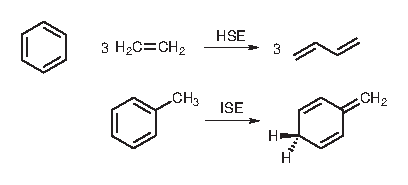
\includegraphics{figures/intro/ase.eps} 
				\caption[]{(top) A homodesmotic reaction for calculating the HSE of benzene; (bottom) the reaction scheme for calculating the ISE of benzene.}
				\label{fig:intro:ase}
			\end{figure}


			The ISE has been evaluated for the annulenes from benzene ([6]-annulene) to [66]-annulene (\autoref{fig:intro:isevspielec}).\autocite{Wannere2003} As ring size increases, ISE-per-electron becomes vanishingly small: for example, [42]-annulene has an ISE-per-electron of \SI{2.3}{\kilo\joule\per\mole}. Put into context, this is about the same as the entropic cost, at room temperature, of freezing a sp\tsup2--sp\tsup2 torsion.\autocite{Mammen1998} This comparison implies that, for large annulenes, the aromatic stabilisation energy becomes vanishingly small compared to the entropic cost of maintaining a regular cyclic geometry necessary for aromaticity.

			\begin{figure}[ht!]
				\centering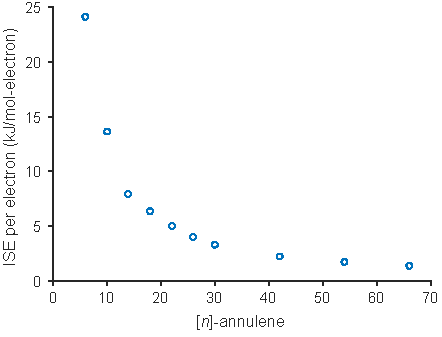
\includegraphics{figures/intro/ise-vs-pielec.pdf} 
				\caption[]{Isomerisation stabilisation energy (ISE) per electron for the annulenes, B3LYP/6-31G*. Data from Wannere and Schleyer.\autocite{Wannere2003}}
				\label{fig:intro:isevspielec}
			\end{figure}



		\subsubsection{Electronic}

			There has been a recent adoption of computational aromaticity metrics which describe electron delocalisation directly, rather than a physical observable such as BLA, or magnetic properties. These metrics have recently been reviewed.\autocite{Feixas2015} Indeed, the ACID method (see Section \ref{sec:intro:rc}) also falls into this category. Without going into too much detail, many electron-delocalisation measures are calculated by evaluating the nature of the electron density at bond critical points and ring critical points (\ltt{i.e.} at the centres of bonds and rings), within the framework of the Quantum Theory of Atoms in Molecules.\autocite{Palusiak2007} In contrast to the other methods presented above, wavefunction analysis is perhaps the most remote from an experimental observable (\ltt{cf.} NMR for NICS, crystallography for structural properties, and calorimetry for stabilisation energies).


	\subsection{Topological effects on aromaticity}

		The annulenes are all monocyclic carbocycles, but molecules can exhibit much broader topological diversity, which has implications for the assignment of aromaticity. In this section we discuss, roughly in order of their appearance in the literature, polycyclic aromaticity and Clar's rule, homoaromaticity, and M\"obius aromaticity.

		\subsubsection{Polycyclic aromaticity}

			Some of the earliest identified aromatic compounds, on the basis of smell, were those comprising fused benzene rings. These molecules exhibit some non-aromatic character in their reactivity: anthracene (\cmpd{anthracene}), comprising three linearly fused benzene rings, undergoes Diels-Alder reaction at the 9,10-positions of the central benzene ring. Phenanthrene (\cmpd{phenanthrene}) has distinctly olefinic chemistry at its 9,10-positions. These observations were rationalised by Clar, who noted that the aromaticity of a polybenzenoid molecule depends on the number, and location, of discrete aromatic sextets of six \pii{}-electrons.\autocite{clar1972aromatic} In anthracene, three resonance structures, each with one sextet, can be drawn; Diels-Alder chemistry at the 9,10-positions offers a product with two Clar sextets (\cmpd{anthYes}), while reaction at either of the terminal benzene rings gives just one Clar sextet (\cmpd{anthNo}). Hence reactivity is exclusively at the 9,10-positions. For phenanthrene (\cmpd{phenanthrene}), the maximum possible number of sextets is two, for the terminal rings, leaving olefinic character in the central ring (\autoref{fig:intro:clar}).\autocite{Sola2013}



			\begin{figure}[ht!]
				\replacecmpd{anthracene}
				\replacecmpd{anthNo}
				\replacecmpd{anthYes}
				\replacecmpd{phenanthrene}
				\replacecmpd{HBC}
				\centering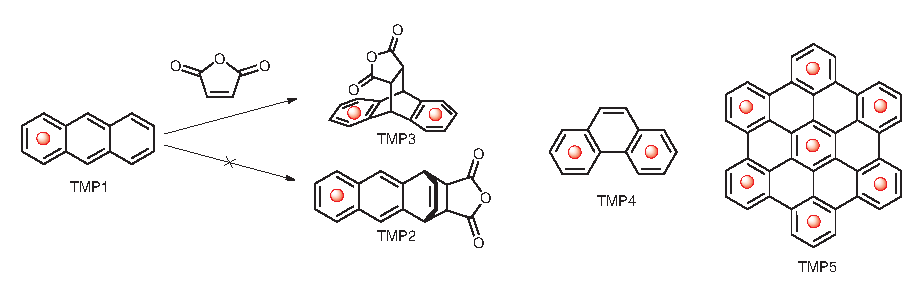
\includegraphics{figures/intro/clar.eps} 
				\caption[]{Examples of polycyclic aromatic hydrocarbons, and the application of Clar's rule to predict and rationalise aromatic character. The red dots denote aromatic sextets.}
				\label{fig:intro:clar}
			\end{figure}

			This idea has been extended to hexabenzocoronene (HBC)\nomenclature{HBC}{Hexabenzocoronene}, which has a maximum of seven aromatic sextets. Spectacularly, the different aromatic and single bond character predicted by Clar's rule is measurable by atomic force microscopy (AFM).\autocite{Gross2012}

			Porphyrins present another example of polycyclic aromaticity: they essentially comprise an [18]-annulene $[4n+2]$ \pii{}-electron pathway appended by two (spectator) ethylene bridges and two aromatic 6 \pii{}-electron pyrroles. Both of these aromatic ring current paths are important to the porphyrin aromaticity, though on an atom-weighted basis the pyrroles contribute more aromatic stabilisation energy.\autocite{Wu2013} %The relative stability conferred by the pyrrole aromaticity is sufficient to give a net aromatic stabilisation to a [20]-annulene (formally antiaromatic) with two fused pyrroles.\autocite{Wu2013}  
			The aromatic stabilisation energy (ASE) calculated by the block-localised wavefunction method to isolate the \pii{}-electron effects shows that the ASE from the macrocyclic [18] \pii{}-electron circuit in the porphyrin is the same as that of an individual 6 \pii{}-electron pyrrole (\SI{\sim 80}{\kilo\joule\per\mole}).\autocite{Wu2013}

		\subsubsection{Homoaromaticity}

			The homoaromatics comprise a different sort of topological perturbation of the monocyclic \pii{}-framework of the annulenes: introduction of an insulating (\ltt{e.g.} \ce{CH2}) interruption. Remarkably, aromaticity and conjugation can persist in charged species despite this disruption. So, the homotropylium cation \cmpd{homoarom} (\ce{C8H9+}, \autoref{fig:intro:aromatics}) is distinctly aromatic, as revealed by the different chemical shifts of protons 8 (inside, \SI{-0.6}{\ppm}) and 8\textprime{} (outside, \SI{5.2}{\ppm}).\autocite{Rosenberg1962,Gleiter2012}

			Homoaromaticity is much rarer for neutral species,\autocite{Gleiter2012} and seems to arise only when the \pii{}-orbitals on either side of the conjugation defect are close enough to effect delocalisation, such as in the theoretical trishomoaromatic molecule \cmpd{trishomoarom} (\autoref{fig:intro:aromatics}).\autocite{Stahl2002}

		\subsubsection{M\"obius aromaticity}

			Heilbronner (1964) predicted that the introduction of a \SI{180}{\degree} phase shift into the aromatic \pii{}-system would reverse H\"uckel's law: such a molecule with $[4n]$ \pii{}-electrons is then aromatic, and $[4n+2]$ \pii{}-electrons becomes antiaromatic.\autocite{Heilbronner1964} Such molecules are known as M\"obius aromatic molecules, for their resemblance to the topological M\"obius strip (\autoref{fig:intro:mobius}).

			\begin{figure}[ht!]
				\centering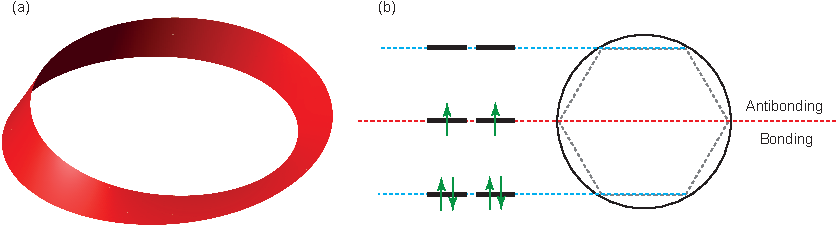
\includegraphics{figures/intro/mobius.pdf} 
				\caption[]{(a) A M\"obius strip. (b) A Frost-Musulin diagram for a hypothetical 6 \pii{}-electron M\"obius molecule.}
				\label{fig:intro:mobius}
			\end{figure}

			The first synthetic example of a M\"obius aromatic molecule was given by Herges and coworkers: the twisted [16]-annulene \cmpd{herges} (\autoref{fig:intro:mobiusstr}) is aromatic.\autocite{Ajami2003} It is possible to introduce two M\"obius twists into a molecule, at which point it reverts back to H\"uckel's aromaticity rules.\autocite{Fowler2006,Rzepa2005} Several examples of expanded porphyrins which exhibit M\"obius aromaticity have been reported by Osuka and co-workers.\autocite{Yoon2009a}



			\begin{figure}[ht!]
				\replacecmpd{herges}
				\centering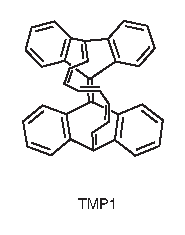
\includegraphics{figures/intro/mobius.eps} 
				\caption[]{Example of M\"obius aromatic compound \cmpd{herges}.\autocite{Ajami2003}}
				\label{fig:intro:mobiusstr}
			\end{figure}


		\subsubsection{Excited state aromaticity}

			In molecules which exhibit excited state (anti)aromaticity (ES(A)A), the electron-counting rules are once again reversed (\autoref{table:intro:arom}).\autocite{Baird1972,Rosenberg2014} The effect has been reported in expanded porphyrins by Osuka and co-workers, and was assigned on the basis of the structure of excited state absorption spectra.\autocite{Sung2015,Oh2016} In their case, an excited state aromatic compound has an absorption spectrum similar to a ground state aromatic analogue, and \ltt{vice versa} for excited state antiaromaticity. A further introduction to excited state aromaticity is given in \autoref{ch:excited-arom}.


			\begin{table}[!ht]
				\centering
				\caption[]{Effect of topology, \pii{}-electron count and electronic state on (anti)aromatic character.}
				\label{table:intro:arom}
				\begin{threeparttable}
					\begin{tabular}{lcccc}
						 & \multicolumn{2}{c}{Ground state} & \multicolumn{2}{c}{Excited state} \\
						 & $4n$ & $4n+2$ & $4n$ & $4n+2$ \\
						 \midrule
						 \textit{H\"uckel} & Antiaromatic & Aromatic & Aromatic & Antiaromatic \\ 
						 \textit{M\"obius} & Aromatic & Antiaromatic & Antiaromatic & Aromatic \\
						\bottomrule
					\end{tabular}
				\end{threeparttable}
			\end{table}


	\section{The limits of electron delocalisation}

		Aromaticity can be considered the limit of electron delocalisation in molecules: the ring-current model leads us to imagine that the \pii{}-electrons are freely circulating around the entire conjugation path. However, cyclic conjugation is not the sole requirement for aromaticity: the cycloparaphenylenes (CPP) and cycloparaphenyleneacetylenes (CPPA) do not exhibit measurable macrocyclic aromaticity around their peripheries,%
%
			\footnote{Taubert \ltt{et al.} have calculated the magnitude of macrocyclic ring currents in [6]-CPP to [11]-CPP and report paratropic and diatropic currents for [6]-CPP and [7]-CPP, respectively. These ring-currents do not significantly affect NICS(0) at the CPP ring centres (\SI{-2.1}{\ppm} and \SI{-1.9}{\ppm} for [6]- and [7]-CPP, respectively). The reversal of the calculated current direction between [6]- and [7]-CPP is surprising because both CPPs are, formally, $[4n]$ all-\textit{cis} annulenes. In contrast, the dianions  ($[4n+2]$ \pii{}-electrons) of all the CPPs studied are aromatic according to NICS(0).\autocite{Taubert2010}} %
		%
		as evidenced by their benzeniod NMR spectra.\autocite{Kawase2007,Jasti2011,Xia2012} Indeed, it is only upon oxidation to the dication that a ring current is observed in [8]-CPP.\autocite{Toriumi2015} Similarly to homoaromaticity in charged molecules, it seems that oxidation disrupts the ground state electronic character (8 isolated benzene rings) and permits enhanced delocalisation (a [32]-annulene dication with 30 \pii{}-electrons). 

		We are led to the inevitable question: if CPP does not exhibit macrocyclic aromaticity, how can porphine be aromatic? Porphine has three sources of aromatic stabilisation, all calculated to be of roughly equal weight (\SI{\sim 80}{\kilo\joule\per\mole} BLW-ASE (block-localised wavefunction)): the [18]-annulene pathway and two pyrroles.\autocite{Wu2013} The pyrrole aromaticity is not entirely `switched off' in favour of the [18]-annulene circuit, since there are still local pyrrolic ring currents. The same calculations predict a BLW-ASE for benzene of about \SI{120}{\kilo\joule\per\mole}, and for isolated pyrrole of about \SI{70}{\kilo\joule\per\mole}.\autocite{Wu2013} 

		There are two key differences between the CPP(A)s and porphine: first, there is much more ASE to be lost (about \SI{50}{\kilo\joule\per\mole}) by (partial) disruption of the local aromaticity of benzene than of pyrrole. Second, in the absence of an [18] \pii{}-electron circulation in porphine, the 12 non-pyrrolic \pii{}-electrons of the circuit are localised: essentially, there is a Pauling resonance argument for delocalising these additional electrons through macrocyclic aromaticity. In contrast, CPP has no localised electrons, and [$n$]-CPPA has a $6n$:$4n$ ratio of aromatic:static electrons. If a macrocyclic ring current were to be established in [$n$]-CPPA, only 4 \pii{}-electrons from each benzene would be involved, immediately negating the electron-counting benefit of including $2n$ acetylene electrons in the macrocyclic aromatic circuit.\autocite{Bleszynski-Jayich2009}

		As will be discussed in the introductions to Chapters \ref{ch:hexacat}, \ref{ch:excited-arom} and \ref{ch:truncnano}, large aromatic molecules are of interest because they may exhibit novel quantum effects, such as a Aharonov-Bohm oscillations of the ring current direction as a function of magnetic field.\autocite{Bleszynski-Jayich2009,Mayor2003} Such oscillations, introduced in more detail in \autoref{ch:hexacat}, could result in magnetic field control of conductance through a molecular junction.\autocite{Hod2006,Rai2011} Intriguingly, at high magnetic fields it has been calculated that molecular ring currents will reverse direction,\autocite{Soncini2004,Tellgren2009} just like the experimental observations in metal rings.\autocite{Chandrasekhar1991}

		Aromaticity and antiaromaticity are predominantly features of molecules with even numbers of electrons. For those with odd-numbers of electrons, such as radical cations and anions, the focus for studies of electron delocalisation is the radical electron/hole, or polaron. As we shall introduce more thoroughly in \autoref{ch:radcat}, the extent of charge (or spin) delocalisation is an important predictor of molecular properties in a device: with long delocalisation lengths, coherent transport becomes possible, preserving the quantum state of an injected electron or hole.\autocite{Heckmann2012} In contrast, shorter delocalisation lengths can still transmit charge over long distances along a molecular wire, through a stepwise hopping process.\autocite{Heckmann2012} Charge delocalisation has been reported to be `extreme' (across up to seven porphyrin units, \SI{7.5}{\nano\metre}) in monoalkyne-linked linear porphyrin oligomer radical cations and anions.\autocite{Susumu2006,Therien2015} Polyfluorenes (\textbf{PF}) have been extensively studied, and seem to have a radical anion delocalisation length of 3--5 fluorene units.\autocite{Takeda2006,Zaikowski2012,Bakalis2014} For poly(3-decylthiophene) (\textbf{P3DT}), the polaron delocalisation length is remarkably long: 11.5 units for an anion, or 8.7 units for a cation,\autocite{Takeda2012} though in terms of spatial extent (\SIrange{4}{5}{\nano\metre}) these distances are similar to those for \textbf{PF}. In contrast, the polaron delocalisation length is limited to 2--3 monomer units in a poly(phenylenevinylene) (\textbf{PPV}) radical anion.\autocite{Nguyen2010,Bakalis2014}

		\begin{figure}[ht!]
			\centering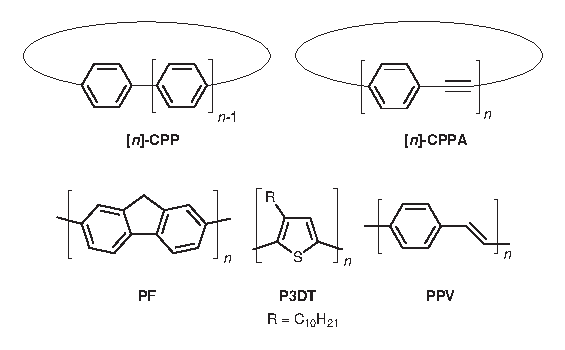
\includegraphics{figures/intro/polymers.eps} 
			\caption[]{Examples of conjugated polymers.}
			\label{fig:intro:polymers}
		\end{figure}

		Charge delocalisation is controlled by two competing effects: the conjugated \pii{}-system efficiently delocalises charge, but its efforts are frustrated by the presence of conjugation breaking defects. These defects can be kinks and twists in the oligomer chain,\autocite{Grozema2002} or can arise from a more dynamic vibrational relaxation following polaron formation: electron-phonon coupling. In this second case, a short segment of the oligomer chain becomes more strongly conjugated (lower BLA) and thus encourages charge localisation within this region.\autocite{Takeda2012} Overall, polaron delocalisation depends on \pii{}-conjugation, oligomer flexibility, and the absence of charge-localising vibrations.


%DFT on PPV. Effect of functional on delocalisation. In all cases singlet > polaron > triplet \autocite{Nayyar2011}

	\section{Prospective}

		The remainder of this thesis starts by considering perhaps the simplest case of delocalisation in butadiyne-linked porphyrin oligomers: the resonance energy of the neutral dimer \lp2 (\autoref{ch:dimer}). The resonance energy is determined from the experimentally determined height of the torsion barrier for rotation of porphyrins around the butadiyne link. \autoref{ch:dimer} also serves to introduce some of the photochemistry of porphyrins. 

		Next, we explore the chemistry of the even \pii{}-cations of the [6]-porphyrin nanoring \cp6 and its template complex \rwt6 (\autoref{ch:hexacat}). Although the nanoring does not exhibit global aromaticity (\ltt{i.e.} around the nanoring circumference) in its neutral oxidation state, after oxidation it is shown to obey H\"uckel's law. \cp6 exhibits aromaticity and antiaromaticity in its 6+ and 4+ oxidation states, respectively. It is even possible to generate the 12+ cation of the nanoring: this oxidation state corresponds to six antiaromatic ([16]-\pii{}) porphyrin subunits, and global (anti)aromaticity is not prominent. These conclusions are developed from DFT and experiment.

		We next turn to an exploration of charge and spin delocalisation in the radical cations of a series of linear (\lp1 to \lp6), cyclic (\cp6 and \rwt6) and tubular (\tubewt{}) porphyrin oligomers (\autoref{ch:radcat}). By using spectroelectrochemistry, DFT, and EPR, we show that the cation is delocalised over just two or three porphyrin units.

		The thesis concludes with two short chapters which each extend the study of aromaticity in porphyrin nanorings. In \autoref{ch:excited-arom} we ask whether porphyrin nanorings exhibit ES(A)A\@. Although DFT suggests that nanorings smaller than \cp8 do have ES(A)A, initial photophysical experiments do not reveal any physical manifestations. In the final chapter (\autoref{ch:truncnano}) we use DFT to calculate the effect of removing a single acetylene (\ce{C2}) unit from \cp6 -- does the nanoring still obey H\"uckel's rules when two \pii{}-electrons are removed, with an accompanying reduction in symmetry? The resulting molecule, with asymmetric conjugation paths, is interesting for studies on quantum interference. This chapter is entirely computational: synthetic efforts towards the truncated nanoring are under way independently. 



%Porphyrin with exocyclic double bonds in the meso positions is non-aromatic: just four aromatic pyrroles but no communication between them, just cross-conjugation.\autocite{Otto1991}

%Porphyrins with a pyridine in the macrocycle are non-aromatic \autocite{Abebayehu2016}
